\chapter{Implementierung des Prototypen}

Das im vorigen Kapitel dargestellte Konzept soll im Weiteren realisiert werden. Dabei wird auf Implementierung oder Probleme innerhalb der einzelnen hierbei involvierten Schritte eingegangen und diese erläutert.

Es wurden viele Open-Source-Bibliotheken verwendet, um den Fokus der Arbeit auf die Neuentwicklung der Lösung zu legen.

Github wurde im Verlauf der Arbeit genutzt, da das Unternehmen der größte Dienstleister für die Bereitstellung von Git-Repositorys ist \cite{Chacon2014}. Neben der Speicherung von Quellcode ist Github ebenfalls eine zentrale Plattform für den Austausch und die Zusammenarbeit von Millionen von Entwicklern. Nicht nur open-source sondern auch closed-source Projekte werden dort gespeichert und mithilfe von Problemverfolgung und Codereviews weiterentwickelt. Für die Verwaltung der Informationen verwendet Github das Versionsverwaltungwerkzeug Git und baut seine Funktionalität und Angebote auf Basis dieser Technologie.

\section{Einschränkungen}
Die zu entwickelnde Software kann nur wie beschrieben verwendet werden, wenn keine effektiven Schutzmaßnahmen implementiert und verwendet wurden.
Folgende Maßnahmen würden das Mitlesen der Kommunikation verhindern.
\begin{enumerate}
    \item Nutzung von \ac{HPKP}
    
    Auf dem Server wird ein für den Client ausgestelltes Zertifikat hinterlegt. Der öffentliche Schlüssel oder der \emph{subjectPublicKeyInfo}, ein weiterer Schlüssel mit Zusatzinformationen über die Verschlüsselung, dieses Zertifikats wird auf dem Client abgespeichert. Anschließend wird dieser gespeicherte Schlüssel mit jeder Anfrage an den Server mitgeschickt. Nachfolgend kann der Server die eingehenden Nachrichten mithilfe der Informationen aus dem Zertifikat verifizieren und sicherstellen, dass sie vom richtigen Ziel kommt \cite{evans_palmer_sleevi_2015}.
    
    \item Der Zertifizierungspfad des SSL-Zertifikats (auch \emph{Chain of Trust} genannt \cite{georgiev2012most}) wird nicht geprüft
    
    Bei Verwendung von TLS ist es möglich, den Client prüfen zu lassen, ob der Server das entsprechende Hersteller-Zertifikat besitzt. Jedes gültige Zertifikat muss von einer \ac{CA} (\emph{Certification Authority}) ausgestellt werden, welche das Vertrauen und eventuell die Identität des Besitzers verifiziert. Jedoch gibt es auch Implementierungen die vom Zertifikat nur die formalen Details und nicht die Herkunft (also die \ac{CA}) prüfen.
    Dies ermöglicht, dass die Kommunikation trotz eines selbst ausgestellten (und somit unverifizierbaren) Zertifikats mit den gleichen Details hergestellt werden kann.
\end{enumerate}


%%%%%%%%%%%%%%%%%%%%%%%%%%%%
%Test Client/Broker implementieren
%%%%%%%%%%%%%%%%%%%%%%%%%%%%
\section{Aufsetzen des externen Client und Broker}
    Da zum Zeitpunkt der Entwicklung keine \ac{IoT}-Geräte zur Verfügung standen, wurden ein virtueller Client und Broker erzeugt, die für die Verifizierung im Labor verwendet wurden.
    Auf diese wird im folgenden Abschnitt eingegangen.

    %Gewählte Sprache für Client und Broker
    Für die Implementierung des virtuellen Clients und externen Brokers bot sich aus folgenden Gründen Python an:
    \begin{itemize}
        \item Die Programmiersprache sollte schnell und mit geringem Aufwand zu verwenden sein.
        \item Sie sollte bereits über eine \ac{MQTT}-Bibliothek verfügen, um das Protokoll nicht selbst interpretieren zu müssen.
        \item Der Client sollte programmierbar und nicht nur konfigurierbar sein.
        \item Die Sprache sollte auf Linux laufen, um eine ressourcensparende Verwendung zu ermöglichen.
        \item Sie sollte ebenfalls auf verschiedenen Betriebssystemen lauffähig (\emph{cross platform}) sein, um auf beliebigen Systemen verwendbar zu sein.
    \end{itemize}
    %https://pdfs.semanticscholar.org/409d/3f740518eafcfaadb054d9239009f3f34600.pdf
    Python ist eine interaktive und objektorientierte Programmiersprache. Sie wird, anders als bei üblichen Programmiersprachen, nicht zuvor kompiliert\footnote{In maschinenlesbare Instruktionen umwandeln.} sondern zur Laufzeit interpretiert.
    Es stehen verschiedene Datenstrukturen aus high-level Programmiersprachen zur Verfügung wie z.B. dynamische Bindungen, automatisches Memory-Management, Klassen und Ausnahmebehandlung. Weiter ist sie eine einfache, leistungsstarke und universelle Programmiersprache, die eine pseudocode ähnlichen Syntax vorweist. \cite{sanner1999python}
        
    %Open-Source Bibliotheken Client/Broker
    Eclipse Paho ist eine quelloffene Implementierung eines Clients nach dem \ac{MQTT}-Standard. Dieser Client ist in verschiedenen Programmiersprachen verfügbar und bringt abhängig von dieser ausgewählte Funktionalitäten mit.
    Das Protokoll \ac{MQTT} in der Version 5 wird aktuell bereits in der Sprache C, jedoch von keiner anderen Implementierung unterstützt. Python unterstützt Version 3 des Standards und alle weiteren Features abgesehen von \emph{Message persistance} und \emph{High availability}, welche jedoch zu Testzwecken nicht benötigt werden. \cite{eclipse_foundation2017}
    Diese Bibliothek vereinfacht das Programmieren der Clients mithilfe der vordefinierten Klassen und Funktionen.
    Aus diesem Grund kann sehr viel konfiguriert und somit auf die gewünschten Anforderungen angepasst werden. 

    HBMQTT ist ebenfalls eine Implementierung des \ac{MQTT}-Standards, allerdings stellt diese Bibliothek auch einen Broker zur Verfügung. Der Vor- und gleichzeitiger Nachteil ist, dass dieses Framework sehr restriktiv und eingeschränkt konfigurierbar ist. Dies erleichtert das aufzusetzen des Brokers, führt jedoch auch dazu, dass Anpassungen nicht ohne Weiteres durchgeführt werden können. \cite{jouanin_2018}
    
%%%%%%%%%%%%%%%%%%%%%%%%%%%%
%Implementieren des Proxys (Backend)
%%%%%%%%%%%%%%%%%%%%%%%%%%%%
\section{Implementierung des Backends}

    Es wurden verschiedene Programmiersprachen für den Proxy verwendet. Diese wurden abhängig der Anforderungen und dem Einsatzgebiet gewählt.
    Der wichtigste Unterschied liegt an der Trennung von Backend (Server- und Logik- Komponenten) und Frontend (Webseite oder User-Interface).
    Zuerst wird auf die Sprache für das Backend eingegangen.
    
%%%%%%%%%%%
%Visual Studio
%%%%%%%%%%%
    Als Entwicklungsumgebung für das Backend wurde Visual Studio 2017 von Microsoft verwendet \cite{microsoft_2019}. Dadurch sind auch die Projektdateien, die in dem Repository \emph{MQTT-Proxy} gefunden werden können, in einem Visual-Studio-Projektfile (Datei mit einer \emph{.sln}-Endung) definiert \cite{eisenschmidt_2019}.
    
%%%%%%%%%%%
%Anforderungen an die Programmiersprache
%%%%%%%%%%%
    \begin{itemize}
        \item Die Sprache muss verschiedene Bibliotheken mitbringen, die Funktionalitäten wie REST-Interface und \ac{MQTT}-Protokoll bereitstellen. Dies ist aufgrund der kurzen Zeit, die für diese Arbeit veranschlagt wurde, notwendig, um alle Features implementieren zu können.
        \item Das Programm muss auf mindestens zwei Plattformen verwendbar sein, um den praktischen Nutzen zu steigern.
        \item Es soll eine bekannte Sprache sein, um eine Weiterentwicklung durch Dritte zu ermöglichen.
        \item Die Programmiersprache muss dem Autor bereits bekannt sein, um die Einarbeitungszeit zu minimieren und eine entsprechende Qualität zu gewährleisten.
    \end{itemize}
%%%%%%%%%%%
%Sprache
%%%%%%%%%%%
    %Welche Sprachen wären basierend darauf möglich/naheliegend gewesen
    Basierend auf diesen Anforderungen stehen Java, C\# und JavaScript zur Auswahl.
    Es wurde sich anschließend aus folgenden Gründen für C\# entschieden.
    %Warum sind die Entwickelt worden? / Vorteile Background
    %Was macht die Programmiersprachen aus? / Schwerpunkt
    \begin{itemize}
        \item Die \ac{IDE} \emph{Visual Studio} und das .NET-Framework sind stark in Windows integriert, wodurch die Verwendung dieser unter Windows erleichtert wird.
        \item Das .NET-Framework besitzt ein Assembly-System, bei dem Bibliotheken in einzelne Dateien ausgelagert und dynamisch geladen werden können.
        \item Es ist kein Linking nötig, da externe Abhängigkeiten zur Laufzeit aufgelöst werden.
        \item Das Paketmanagement-System \emph{NuGet} ermöglicht eine schnelle und einfache Verwaltung sowie Einbindung externer Bibliotheken.
    \end{itemize}
    
    
%%%%%%%%%%%
%Nuget %https://link.springer.com/book/10.1007%2F978-1-4302-4192-8
%%%%%%%%%%%
    \emph{NuGet} wurde aus den folgenden Gründen ausgewählt, welche ebenfalls von Balliauw et al. beschrieben werden \cite{balliauw2012pro}.
    Der sogenannte Paket-Manager unterstützt bei der Verwaltung von Abhängigkeiten, wie zum Beispiel Bibliotheken, und unterstützt den Nutzer bei Versionsproblemen von Abhängigkeiten. Versionsprobleme treten dann auf, wenn Bibliotheken Abhängigkeiten mit einer Version < X und eine weitere Bibliothek Version > X benötigen. Ein weiterer oft auftretender Fall ist, dass beim Aktualisieren einer Bibliothek die benötigte Version für die Abhängigkeiten erhöht aber nicht ebenfalls aktualisiert wird. Die Folge ist eine defekte Abhängigkeit für die Bibliothek, also ein nicht kompilierbarer Zustand, wodurch das Programm nicht ausführbar ist. Zusätzlich übernimmt \emph{NuGet} auch die Installation durch Suchen, Installieren und Aktualisieren oder Entfernen von gewünschten Paketen. Ein weiterer Vorteil ist, dass der Quellcode öffentlich verfügbar ist und das Tool somit weiter angepasst oder verändert werden kann.
    
%%%%%%%%%%%
%Bibliothek
%%%%%%%%%%%
    NewsoftJSON ist ein quelloffenes Framework für die Serialisierung und Deserialisierung von .NET-Framework-Objekten \cite{newton_king_2013}.
    Heinzl beschreibt Serialisierung als \glqq[...] die Zerlegung des Status eines Objekts in ein Bytearray.\grqq{} \cite{Heinzl2005}. Allerdings ist es auch möglich, dieses Bytearray als strukturierten Text anzeigen zu lassen.
    Dies ermöglicht, ein Nachrichtenobjekt an das Frontend zu übertragen und es dort anschließend wieder darstellen zu lassen.
    
    MQTTNet ist eine quelloffene Implementierung des \ac{MQTT}-Standards in C\# unter der MIT-Lizenz\footnote{Github beschreibt die Lizenz als einfache freizügige Lizenz mit nur wenigen Einschränkungen wie dem Erhalt von Urheberrechts- und Lizenzhinweisen. Änderungen und größere Werke können unter anderen Lizenzbedingungen und ohne Quellcode verbreitet werden. \cite{github_inc_2019}}.
    Da die Bibliothek MQTTnet \cite{chkr1011_2018}, welche in dieser Arbeit verwendet wird, die Bridge-Funktionalität nicht besitzt, ist es notwendig, sie selbst zu implementieren. Um das gleiche Ergebnis wie bei einer Bridge zu erreichen, muss an den Broker eine Client-Komponente angeschlossen werden, die die Kommunikation nach außen steuert und die Antworten weiter verarbeitet. 
    
    WebSocketSharp ist eine C\#-Implementierung des WebSocket-Protokolls und unterstützt sowohl den Client als auch die Bereitstellung des Servers.
    
    Grapevine ist eine .NET-Bibliothek die zwei Probleme verfolgt: Das einfache Einbinden eines REST- und HTTP-Servers und die einfache Verwendung von REST-Ressourcen.
    Der Fokus liegt dabei auf der Bereitstellung von Ressourcen über HTTP oder REST für Programme, die einen anderen Schwerpunkt haben und dies nur als Zusatzfunktion benötigen.
    
%%%%%%%%%%%%%%%%%%%%%%%%%%%%
%Implementieren des Proxys (Frontend)
%%%%%%%%%%%%%%%%%%%%%%%%%%%%
\section{Implementierung des Frontends}
    
    Nun wird auf die Programmiersprache für das Frontend, also die Oberfläche eingegangen.
    
%%%%%%%%%%%
%Visual Studio Code
%%%%%%%%%%%
    %https://proquestcombo.safaribooksonline.com/9781484242247
    Zum Entwickeln des Frontends, also der Weboberfläche mit der Nutzer interagieren und die Applikation steuern können, wurde \emph{Visual Studio Code} verwendet \cite{microsoft_2016}.
    
%%%%%%%%%%%
%Anforderungen an die Programmiersprache
%%%%%%%%%%%
Die Programmiersprache soll folgenden Anforderungen entsprechen:
    \begin{itemize}
        \item Es muss möglich sein, einzelne Inhalte auf der Webseite dynamisch, also ohne Aktualisierung, austauschen zu können.
        \item Wenn neue abgefangene Nachrichten im Proxy verfügbar sind, sollen diese automatisch an das Frontend weitergegeben werden und das Datenmodell der Oberfläche automatisch aktualisieren.
        \item Die Oberfläche soll aus Komponenten bestehen und mithilfe dieser soll ein modularer und strukturierter Aufbau ermöglichen werden.
        \item Funktionalitäten und Ausprägungen von Komponenten sollen gekapselt sein. Dies ermöglicht die Wiederverwendung von Komponenten und legt ihre Verantwortlichkeiten und Aufgaben fest.
    \end{itemize}
    
%%%%%%%%%%%
%Welche Sprachen wären basierend darauf möglich/naheliegend gewesen
%%%%%%%%%%%
    Durch die existierenden Anforderungen hat sich JavaScript als passend herausgestellt. Dadurch, dass verschiedene Frameworks und Erweiterungen für JavaScript existieren, werden im Folgenden die ausgewählten Frameworks vorgestellt.
    
%%%%%%%%%%%
%Warum Vue.js
%%%%%%%%%%%
    Vue.js wurde ursprünglich für schnelles Prototyping von Webseiten entwickelt, ist mit der Zeit eine populäre Webtechnologien geworden \cite{you2018vue,stack_overflow_2019}. Neben Angular und React, stellt es eine Alternative zum schnellen und leichtgewichtigen Entwickeln mit \ac{MVVM}-Architekturmuster dar. Dies ermöglicht die Wiederverwendung von Code durch Nutzung von Komponenten. Durch die bidirektionale Datenbindung ist es möglich, Änderungen im Clientmodel direkt ohne Aktualisierung anzeigen zu lassen. In der entgegengesetzten Richtung werden die Informationen, welche zum Beispiel in Eingabefeldern bearbeitet werden können, direkt im Clientmodel abgespeichert. Ein Vorteil ist die direkte Abbildung vom Datenmodel (also Datenstruktur) zum ViewModel. Dies ermöglicht auch eine Trennung von UI- und Backendentwicklung da getrennt entwickelt werden kann ohne Informationen in Bereichen der anderen abändern zu müssen. \cite{filipova_2016}
    %%%%%%%%%%%%%%%%%%%%%%%%%%%%%%%%%%%%%%%
    % Danke an Moritz für die Infos \.A./ %
    %%%%%%%%%%%%%%%%%%%%%%%%%%%%%%%%%%%%%%%
    
%%%%%%%%%%%
%Bibliothek
%%%%%%%%%%%
    Als Bibliothek wurde Bootstrap-Vue gewählt, um schnell anpassbare Oberflächen erstellen zu können.
    Laut Morehouse \cite{morehouse_2019} ist sie die umfassendste Implementierung von Bootstrap in der Version 4 für Vue.js.
    Bootstrap ist ein quelloffenes Framework, welches fertige Vorlagen und Komponenten für die Erstellung von Webseiten bereitstellt \cite{otto_thornton_2019}. Der Unterschied zwischen Bootstrap und Bootstrap-Vue besteht darin, dass die vorhandenen Elemente nun als Komponenten in Vue vorhanden sind und somit nicht der ursprüngliche \ac{HTML}-Code\footnote{\ac{HTML} ist die Auszeichnungssprache für das \ac{WWW} \cite{w3c_2017}. Was bedeutet, dass es die grundlegende Sprache für das Erstellen von Webseiten ist.} geschrieben werden muss. Diese Informationen werden automatisch mithilfe der Vue Komponenten generiert.
        
%%%%%%%%%%%%%%%%%%%%%%%%%%%%
%Kommunikation mit Firewall
%%%%%%%%%%%%%%%%%%%%%%%%%%%%
\section{Umsetzung des MITM-Proxys}
    %MITM (APR Spoof, DNS, ICMP, FW)
    Es gibt verschiedene Techniken und Möglichkeiten, die Kommunikation so zu verändern, dass ein drittes Gerät die übertragenen Nachrichten mitlesen kann. Ein solches Konzept ist auch unter dem Namen \emph{Man in the Middle} bekannt.
    
    Eine der Möglichkeiten, mit denen die Verbindung vom Client direkt zum Broker aufgebaut werden kann, wird auch in dieser Arbeit umgesetzt.
    Mithilfe der Portweiterleitung der Firewall \emph{OPNSense} wurden Netzwerkpakete des \ac{IoT}-Gerätes an den Proxy umgeleitet. Hierzu wurde eine Regel erzeugt (siehe \ref{fig:firewall_rule}), die das \emph{source}-Attribut jedes eintreffenden Pakets mit der IP-Adresse des Gerätes und dem Standard-Port 1883 vergleicht. Bei Übereinstimmung wird das \emph{destination}-Attribut umgeschrieben um die Pakete anschließend an den Proxy weiterzuleiten.
    \begin{figure}[h]%h=direkt danach t=top b=bottom
        \centering
        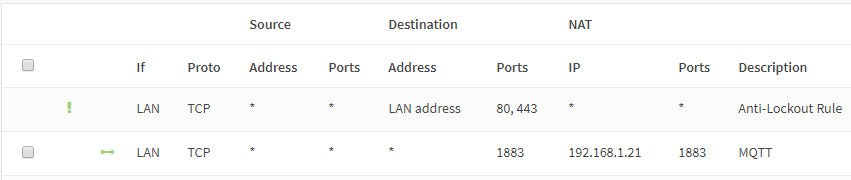
\includegraphics[width=14cm]{tex/bilder/5_implementierung/firewall.PNG}
        \captionof{figure}{Firewall-Regel zum Umleiten der MQTT-Pakete}
        \label{fig:firewall_rule}
    \end{figure}
    
\subsubsection{Zusammenfassung}
    Dieses Kapitel zeigt, wie die Software implementiert wurde und welche dafür notwendigen Bibliotheken eingesetzt wurden. Die Implementierung verwendet, im Gegensatz zu den, sonst restriktiven Umständen geschuldeten, üblichen \ac{MITM}-Methodiken, eine Firewall zur Weiterleitung der Pakete. Dies war durch die vollständige Kontrolle des Netzwerks möglich und erwies sich als komfortable und zuverlässige Lösung.